\documentclass[aspectratio=169, professionalfonts]{beamer}

\usetheme{Szeged}
\usecolortheme{dolphin}

\usepackage{amsmath, amssymb, bm}
\usepackage{tikz}
\usetikzlibrary{positioning, arrows.meta, decorations.pathreplacing, calc}
\usepackage{pgfplots}
\pgfplotsset{compat=1.18}

\def\R{\mathbb{R}}
\def\E{\mathbb{E}}

\definecolor{mantis}{RGB}{0, 105, 62}

\setbeamercolor{frametitle}{fg=white, bg=mantis}
\setbeamercolor{title}{fg=white, bg=mantis}
\setbeamercolor{structure}{fg=mantis}
\setbeamercolor{block title}{bg=mantis, fg=white}
\setbeamercolor{block body}{bg=mantis!10}

\title{The Transformer}
\subtitle{Attention Is All You Need}
\author{Lebnet Tech Fellows Program}
\date{}

\begin{document}

% ------------------------------------------------------------------
\begin{frame}
\titlepage
\end{frame}

% ------------------------------------------------------------------
\begin{frame}{Roadmap}
\tableofcontents
\end{frame}

% ==================================================================
\section{The Problem: Sequence Modelling}
% ==================================================================

% ------------------------------------------------------------------
\begin{frame}{Language Modelling}

Input: a sequence of discrete tokens
$w_1, w_2, \ldots, w_T$ from a vocabulary
$\mathcal{V} = \{1,\ldots,V\}$.

\bigskip

By the chain rule of probability:
$$p(w_1,\ldots,w_T)
  = \prod_{t=1}^{T} p(w_t \mid w_1,\ldots,w_{t-1})$$

So modelling sequences reduces to modelling the conditional
$p(w_t \mid w_{1:t-1})$.

\bigskip

\textbf{Goal:} learn $f_\Theta : \mathcal{V}^* \to [0,1]^V$
that predicts the next token given all preceding tokens.

\bigskip

The \textbf{transformer} is the architecture for $f_\Theta$.
It can attend to the \emph{entire} preceding context.

\end{frame}

% ==================================================================
\section{Embedding and Position}
% ==================================================================

% ------------------------------------------------------------------
\begin{frame}{Token Embedding}

Tokens are integers; we cannot differentiate with respect to them.

\bigskip

\begin{block}{Embedding Matrix $\mathbf{E} \in \R^{V \times d}$}
The embedding of token $w_t$ is the $w_t$-th row of $\mathbf{E}$:
$$\mathbf{e}_t = \mathbf{E}[w_t] \in \R^{1 \times d}$$
Equivalently: one-hot $\mathbf{o}_t$ times $\mathbf{E}$ (a row lookup).
\end{block}

\bigskip

$\mathbf{E}$ is \textbf{learned}: tokens that play similar roles get
similar embeddings. $d$ is the model dimension (e.g.\ 512, 4096, 12288).

\end{frame}

% ------------------------------------------------------------------
\begin{frame}{Positional Encoding}

The embedding depends only on token identity, not position.
But order matters: ``dog bites man'' $\ne$ ``man bites dog''.

\bigskip

\textbf{Fix:} add a position signal to each embedding:
$$\mathbf{x}_t = \mathbf{E}[w_t] + \mathbf{P}[t]$$

Vaswani et al.\ used deterministic sinusoids at different frequencies:
\begin{align*}
\mathbf{P}[t,\,2k]   &= \sin\!\bigl(t / 10000^{2k/d}\bigr) \\
\mathbf{P}[t,\,2k{+}1] &= \cos\!\bigl(t / 10000^{2k/d}\bigr)
\end{align*}

Each position gets a unique signature. The full input to block~1:
$$\mathbf{X} = \mathbf{X}_\text{emb} + \mathbf{P}_{1:N}
  \in \R^{N \times d}$$

\end{frame}

% ==================================================================
\section{Attention}
% ==================================================================

% ------------------------------------------------------------------
\begin{frame}{Motivation}

\emph{``The chicken didn't cross the road because \textbf{it} was too
tired.''}

\bigskip

To represent ``it'', we need to look at other tokens and decide
which ones are relevant.

\bigskip

\textbf{Idea:} compute a weighted sum of all preceding representations:
$$\mathbf{a}_i = \sum_{j \le i} \alpha_{ij}\,\mathbf{x}_j,
  \qquad \alpha_{ij} \ge 0,
  \quad \sum_{j \le i}\alpha_{ij} = 1$$

The constraint $j \le i$ is the \textbf{causal mask}: we cannot look
at future tokens (they don't exist yet at generation time).

\end{frame}

% ------------------------------------------------------------------
\begin{frame}{Queries, Keys, and Values}

Using $\mathbf{x}_i$ for all three roles (query, key, value) is
too restrictive. Separate them with learned projections:

\begin{align*}
\mathbf{q}_i &= \mathbf{x}_i\,\mathbf{W}^Q
  &&\text{``what am I looking for?''} \\
\mathbf{k}_i &= \mathbf{x}_i\,\mathbf{W}^K
  &&\text{``what do I contain?''} \\
\mathbf{v}_i &= \mathbf{x}_i\,\mathbf{W}^V
  &&\text{``what info do I provide?''}
\end{align*}

\begin{block}{Scaled Dot-Product Attention}
\vspace{-6pt}
$$\alpha_{ij}
  = \frac{\exp(\mathbf{q}_i \cdot \mathbf{k}_j / \sqrt{d_k})}
         {\sum_{m \le i}\exp(\mathbf{q}_i \cdot \mathbf{k}_m / \sqrt{d_k})},
  \qquad
  \mathbf{a}_i = \sum_{j \le i}\alpha_{ij}\,\mathbf{v}_j$$
\vspace{-6pt}
\end{block}

\smallskip

Dividing by $\sqrt{d_k}$ keeps score variance at $\sim\!1$,
preventing softmax saturation.

\end{frame}

% ------------------------------------------------------------------
\begin{frame}{The Causal Mask}

In matrix form for all $N$ positions at once:
$$\text{Attention}(\mathbf{Q},\mathbf{K},\mathbf{V})
  = \text{softmax}\!\left(
    \frac{\mathbf{Q}\mathbf{K}^\top}{\sqrt{d_k}} + \mathbf{M}
  \right)\mathbf{V}$$

where $M_{ij} = 0$ if $j \le i$, and $-\infty$ otherwise.

\begin{center}
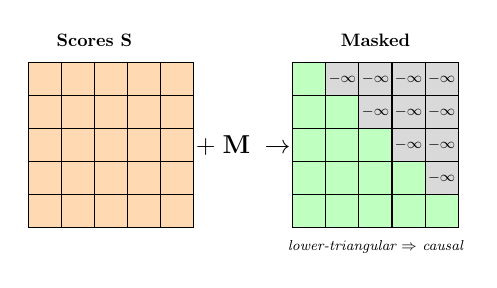
\begin{tikzpicture}[scale=0.42, every node/.style={scale=0.65}]
    \node[above] at (2,5.3) {\textbf{Scores $\mathbf{S}$}};
    \foreach \i in {0,...,4} {
        \foreach \j in {0,...,4} {
            \fill[orange!30] (\j,4-\i) rectangle (\j+1,5-\i);
            \draw (\j,4-\i) rectangle (\j+1,5-\i);
        }
    }
    \node at (6.5,2.5) {\Large $+\;\mathbf{M}\;\to$};
    \node[above] at (10.5,5.3) {\textbf{Masked}};
    \foreach \i in {0,...,4} {
        \foreach \j in {0,...,4} {
            \pgfmathparse{int(\j<=\i)}
            \ifnum\pgfmathresult=1
                \fill[green!25] (8+\j,4-\i) rectangle (9+\j,5-\i);
                \draw (8+\j,4-\i) rectangle (9+\j,5-\i);
            \else
                \fill[gray!30] (8+\j,4-\i) rectangle (9+\j,5-\i);
                \draw (8+\j,4-\i) rectangle (9+\j,5-\i);
                \node[font=\footnotesize] at (8.5+\j,4.5-\i) {$-\infty$};
            \fi
        }
    }
    \node[below, font=\footnotesize\itshape] at (10.5,-0.2)
      {lower-triangular $\Rightarrow$ causal};
\end{tikzpicture}
\end{center}

\smallskip

Cost: $O(N^2 d_k)$ (quadratic in sequence length).

\end{frame}

% ==================================================================
\section{Multi-Head Attention}
% ==================================================================

% ------------------------------------------------------------------
\begin{frame}{Multiple Attention Heads}

Tokens relate in many ways (syntax, coreference, semantics).
A single head can only learn one pattern.

\bigskip

\begin{block}{Multi-Head Attention}
Run $A$ independent heads, each with its own
$\mathbf{W}^{Qc},\mathbf{W}^{Kc},\mathbf{W}^{Vc}$:
$$\text{MultiHead}(\mathbf{X})
  = \bigl[\text{head}^1 \;\|\; \cdots \;\|\;
          \text{head}^A\bigr]\,\mathbf{W}^O$$
\end{block}

\begin{itemize}
  \item Each head operates in a $d/A$-dimensional subspace
  \item Set $d_k = d_v = d/A$ so concatenation returns shape
        $[N \times d]$
  \item Original transformer: $d=512$, $A=8$, $d_k=64$
\end{itemize}

\end{frame}

% ==================================================================
\section{The Transformer Block}
% ==================================================================

% ------------------------------------------------------------------
\begin{frame}{Residual Connections and LayerNorm}

After each sub-layer (attention or FFN):

\begin{columns}[c]
\column{0.5\textwidth}

\textbf{Residual connection:}
$$\mathbf{x}' = f(\mathbf{x}) + \mathbf{x}$$

Gradient is $\mathbf{I} + \frac{\partial f}{\partial\mathbf{x}}$:
always at least the identity. Solves vanishing gradients.

\bigskip

\textbf{LayerNorm} (per token):
$$\text{LN}(\mathbf{x})
  = \gamma \odot \frac{\mathbf{x}-\mu}{\sigma+\epsilon} + \beta$$

Normalises each token's $d$-dim vector to zero mean, unit variance.

\column{0.5\textwidth}
\begin{center}
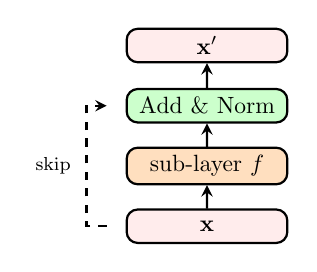
\begin{tikzpicture}[>=stealth, scale=0.85, every node/.style={scale=0.85},
    block/.style={draw, rounded corners, minimum width=2.4cm,
                  minimum height=0.5cm, thick}]
    \node[block, fill=pink!30] (input) at (0,0) {$\mathbf{x}$};
    \node[block, fill=orange!25] (f) at (0,0.9) {sub-layer $f$};
    \node[block, fill=green!20] (an) at (0,1.8) {Add \& Norm};
    \node[block, fill=pink!30] (out) at (0,2.7) {$\mathbf{x}'$};
    \draw[->, thick] (input) -- (f);
    \draw[->, thick] (f) -- (an);
    \draw[->, thick] (an) -- (out);
    \draw[->, thick, dashed] (-1.5,0) -- (-1.8,0)
      -- (-1.8,1.8) -- (-1.5,1.8);
    \node[font=\footnotesize] at (-2.3,0.9) {skip};
\end{tikzpicture}
\end{center}
\end{columns}

\end{frame}

% ------------------------------------------------------------------
\begin{frame}{Feed-Forward Network}

A two-layer MLP applied \textbf{independently} to each position:
$$\text{FFN}(\mathbf{x})
  = \text{ReLU}(\mathbf{x}\,\mathbf{W}_1 + \mathbf{b}_1)\,
    \mathbf{W}_2 + \mathbf{b}_2$$

\begin{itemize}
  \item $\mathbf{W}_1 \in \R^{d \times d_\text{ff}}$,
        $\mathbf{W}_2 \in \R^{d_\text{ff} \times d}$
        with $d_\text{ff} = 4d$
  \item Expands to $4d$, applies nonlinearity, compresses back to $d$
  \item No interaction between positions (attention does that)
\end{itemize}

\end{frame}

% ------------------------------------------------------------------
\begin{frame}{One Block, Repeated $L$ Times}

\begin{columns}[c]
\column{0.38\textwidth}
\begin{center}
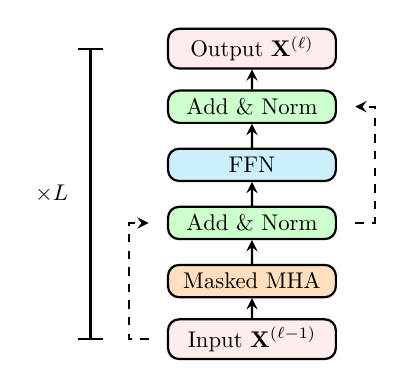
\begin{tikzpicture}[>=stealth, scale=0.82, every node/.style={scale=0.82},
    block/.style={draw, rounded corners, minimum width=2.6cm,
                  minimum height=0.5cm, thick}]
    \node[block, fill=pink!30] (input) at (0,0)
      {Input $\mathbf{X}^{(\ell-1)}$};
    \node[block, fill=orange!25] (mha) at (0,0.9)
      {Masked MHA};
    \node[block, fill=green!20] (an1) at (0,1.8)
      {Add \& Norm};
    \node[block, fill=cyan!20] (ffn) at (0,2.7)
      {FFN};
    \node[block, fill=green!20] (an2) at (0,3.6)
      {Add \& Norm};
    \node[block, fill=pink!30] (output) at (0,4.5)
      {Output $\mathbf{X}^{(\ell)}$};
    \draw[->, thick] (input) -- (mha);
    \draw[->, thick] (mha) -- (an1);
    \draw[->, thick] (an1) -- (ffn);
    \draw[->, thick] (ffn) -- (an2);
    \draw[->, thick] (an2) -- (output);
    \draw[->, thick, dashed] (-1.6,0) -- (-1.9,0)
      -- (-1.9,1.8) -- (-1.6,1.8);
    \draw[->, thick, dashed] (1.6,1.8) -- (1.9,1.8)
      -- (1.9,3.6) -- (1.6,3.6);
    \draw[thick] (-2.5,0) -- (-2.5,4.5);
    \draw[thick] (-2.7,0) -- (-2.3,0);
    \draw[thick] (-2.7,4.5) -- (-2.3,4.5);
    \node[font=\normalsize] at (-3.1,2.25) {$\times L$};
\end{tikzpicture}
\end{center}

\column{0.62\textwidth}

In pre-norm convention:
\begin{align*}
\mathbf{O}^{(\ell)} &= \mathbf{X}^{(\ell-1)}
  + \text{MHA}\!\bigl(\text{LN}(\mathbf{X}^{(\ell-1)})\bigr) \\[4pt]
\mathbf{X}^{(\ell)} &= \mathbf{O}^{(\ell)}
  + \text{FFN}\!\bigl(\text{LN}(\mathbf{O}^{(\ell)})\bigr)
\end{align*}

Input and output are both $[N \times d]$
$\Rightarrow$ blocks stack.

\smallskip

\textbf{Params per block:} $12\,d^2$
($4d^2$ attention + $8d^2$ FFN).

Total: $N_\text{params} \approx 12\,L\,d^2$.

\smallskip

{\small GPT-3: $L\!=\!96$, $d\!=\!12288$
$\Rightarrow$ $\sim$175B params.}
\end{columns}

\end{frame}

% ==================================================================
\section{Output Head}
% ==================================================================

% ------------------------------------------------------------------
\begin{frame}{From Hidden State to Next Token}

After $L$ blocks + final LayerNorm, take the last token's
representation $\mathbf{h}_N \in \R^d$.

\bigskip

\textbf{Unembedding} (weight-tied with $\mathbf{E}$):
$$\mathbf{u} = \mathbf{h}_N\,\mathbf{E}^\top \in \R^V
  \qquad\text{(logits)}$$

\textbf{Softmax}:
$$p(w_{N+1} = k \mid w_{1:N})
  = \frac{\exp(u_k)}{\sum_j \exp(u_j)}$$

\bigskip

Tokens whose embeddings are close to $\mathbf{h}_N$ get high
probability. Weight tying halves the vocabulary parameters
and acts as a regulariser.

\end{frame}

% ==================================================================
\section{Training and Generation}
% ==================================================================

% ------------------------------------------------------------------
\begin{frame}{Training: Cross-Entropy Loss}

At every position $t$, the model predicts $p(\cdot \mid w_{1:t})$.
The loss is:
$$\mathcal{L} = -\frac{1}{T}\sum_{t=1}^{T}
  \log p_\Theta(w_{t+1} \mid w_{1:t})$$

\bigskip

\begin{itemize}
  \item Minimised via Adam + backpropagation through all $L$ blocks
  \item Thanks to the causal mask, \textbf{all positions are computed
        in parallel} (unlike RNNs)
  \item This is the key advantage: massive parallelism during training
\end{itemize}

\end{frame}

% ------------------------------------------------------------------
\begin{frame}{Generation: Autoregressive Sampling}

Given a prompt $w_{1:N}$, generate one token at a time:

\begin{enumerate}
  \item Forward pass $\to$ logits $\to$ softmax $\to$ sample $w_{N+1}$
  \item Append $w_{N+1}$ to the context, repeat
  \item Stop at end-of-sequence token or max length
\end{enumerate}

\bigskip

\textbf{Sampling strategies:}

\begin{itemize}
  \item \textbf{Greedy:} $w_{t+1} = \arg\max_k p_k$
        (deterministic, repetitive)
  \item \textbf{Top-$k$:} keep $k$ most probable, renormalise, sample
  \item \textbf{Top-$p$ (nucleus):} keep smallest set with
        cumulative prob $\ge p$, renormalise, sample
\end{itemize}

\end{frame}

% ==================================================================
\section{The Big Picture}
% ==================================================================

% ------------------------------------------------------------------
\begin{frame}{Recap: The Complete Forward Pass}

\begin{enumerate}
  \item \textbf{Embed + Position:}
    $\mathbf{x}_t = \mathbf{E}[w_t] + \mathbf{P}[t]$
  \item \textbf{$L$ Transformer Blocks}, each:
    \begin{itemize}
      \item Masked multi-head attention (mix information across positions)
      \item Add \& LayerNorm
      \item Feed-forward network (process each position independently)
      \item Add \& LayerNorm
    \end{itemize}
  \item \textbf{Final LayerNorm}
  \item \textbf{Unembedding + Softmax:}
    $\mathbf{p} = \text{softmax}(\mathbf{h}_N\,\mathbf{E}^\top)$
\end{enumerate}

\bigskip

\begin{alertblock}{Key design principles}
\begin{itemize}
  \item Attention = the \emph{only} cross-position operation
  \item Residuals + norms = stable gradient flow through depth
  \item Causal mask = parallel training, autoregressive generation
\end{itemize}
\end{alertblock}

\end{frame}

% ------------------------------------------------------------------
{
\setbeamercolor{background canvas}{bg=mantis}
\setbeamercolor{normal text}{fg=white}
\usebeamercolor[fg]{normal text}
\begin{frame}[c]
\centering
\Huge\textbf{Questions?}
\end{frame}
}

\end{document}
